\section*{Приборы и принадлежности}

Стенд для сборки измерительной цепи; два
источника с различными ЭДС; миллиамперметр и вольтметр; переменный
резистор. 

Схема установки на рис. \ref{schema}

\begin{figure}[hpt!]
	\centering
	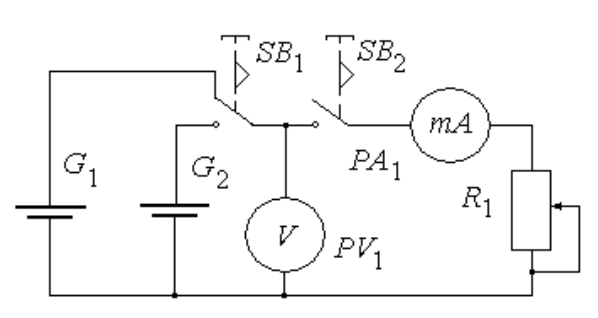
\includegraphics[width=0.6\linewidth]{photo/schema}
	\caption{Схема установки}
	\label{schema}
\end{figure}

Переключателем SB1 источники G1 и G2 с различными ЭДС и
внутренними сопротивлениями могут быть поочередно подключены к
нагрузке R1. Ток I и напряжение Ue на резисторе R1 измеряют
миллиамперметром PA1 и вольтметром PV1. Режим разомкнутой цепи
осуществляется отключением нагрузки кнопкой SB2; показание вольтметра
при этом равно ЭДС источника. 
